% ==========================================================================
% INFO 4617 Web Data Science -- Week 13: AI & Language-Model APIs (Chapter 13)
% Build:  latexmk -pdf week-13.tex   (from this folder; no env vars needed)
% (or run `make` from the slides/ directory to build every deck)
% ==========================================================================
\documentclass[9pt,aspectratio=169]{beamer}
% Resolve the shared theme/preamble in ../common/ when compiling this
% file directly from its own folder (no TEXINPUTS needed).
\makeatletter\def\input@path{{../common/}}\makeatother
% ==========================================================================
% Shared preamble for INFO 4617 Web Data Science weekly lecture decks
% Based on the Gotham beamer theme (vendored in this directory).
% Each week's slides.tex does:  % ==========================================================================
% Shared preamble for INFO 4617 Web Data Science weekly lecture decks
% Based on the Gotham beamer theme (vendored in this directory).
% Each week's slides.tex does:  % ==========================================================================
% Shared preamble for INFO 4617 Web Data Science weekly lecture decks
% Based on the Gotham beamer theme (vendored in this directory).
% Each week's slides.tex does:  \input{preamble}  (with common/ on TEXINPUTS)
% then sets \title/\subtitle/\author/\date and \begin{document}.
% ==========================================================================

\usetheme{gotham}

\usepackage{fbb}
\usepackage{booktabs}
\usepackage{graphicx}
\usepackage{tikz}
\usepackage{xcolor}
\usepackage{multirow}
\usepackage{listings}
\usetikzlibrary{positioning, arrows.meta, shapes}

% Bibliography
\usepackage[style=authoryear,
            backend=biber,
            maxcitenames=1,
            uniquename=false,
            uniquelist=false]{biblatex}
\addbibresource{bibliography.bib}

\gothamset{sectiontocframe default=off}

% ------------------------------------------------------------------ colors
\definecolor{cugold}{HTML}{CFB87C}
\definecolor{tab-red}{HTML}{E15759}
\definecolor{tab-orange}{HTML}{F28E2B}
\definecolor{tab-blue}{HTML}{4E79A7}
\definecolor{tab-cyan}{HTML}{76B7B2}
\definecolor{tab-green}{HTML}{59A14F}
\definecolor{tab-yellow}{HTML}{EDC948}
\definecolor{tab-purple}{HTML}{B07AA1}
\definecolor{tab-pink}{HTML}{FF9DA7}
\definecolor{tab-brown}{HTML}{9C755F}
\definecolor{tab-gray}{HTML}{BAB0AC}

\setbeamercolor{frametitle}{fg=black, bg=cugold}
\setbeamercolor{progress bar}{fg=cugold, bg=cugold!20}

\setbeamercolor{block title alerted}{fg=black, bg=cugold}
\setbeamercolor{block body alerted}{fg=black, bg=cugold!10}

% ------------------------------------------------------------------ footline
\setbeamertemplate{footline}{
  \begin{beamercolorbox}[wd=\paperwidth,ht=2.5ex,dp=1ex,right]{footline}
    {\footnotesize \insertframenumber{} of \inserttotalframenumber}
    \hspace*{2ex}
  \end{beamercolorbox}
}

% ------------------------------------------------------------------ helpers
\newcommand{\bottomcite}[1]{
    \vspace*{\fill}
    \vspace{-\baselineskip}
    {\tiny
    \rule{\textwidth}{0.3pt}\\
    #1
    }
    \vspace{0.5ex}
}

% Consistent code styling for the Wednesday "applied notebook" frames.
\lstdefinestyle{wds}{
    basicstyle=\ttfamily\scriptsize,
    keywordstyle=\color{tab-blue}\bfseries,
    commentstyle=\color{tab-green},
    stringstyle=\color{tab-orange},
    showstringspaces=false,
    breaklines=true,
    columns=fullflexible,
    language=Python,
    aboveskip=0.4em,
    belowskip=0.4em,
}
\lstset{style=wds}

% \dayband{Day}{Topic} -- a lightweight section divider label used to mark
% Monday / Wednesday / Friday within a week's deck.
\newcommand{\dayband}[2]{{\large\textbf{#1}}\;\textcolor{tab-gray}{\textbar}\;#2}
  (with common/ on TEXINPUTS)
% then sets \title/\subtitle/\author/\date and \begin{document}.
% ==========================================================================

\usetheme{gotham}

\usepackage{fbb}
\usepackage{booktabs}
\usepackage{graphicx}
\usepackage{tikz}
\usepackage{xcolor}
\usepackage{multirow}
\usepackage{listings}
\usetikzlibrary{positioning, arrows.meta, shapes}

% Bibliography
\usepackage[style=authoryear,
            backend=biber,
            maxcitenames=1,
            uniquename=false,
            uniquelist=false]{biblatex}
\addbibresource{bibliography.bib}

\gothamset{sectiontocframe default=off}

% ------------------------------------------------------------------ colors
\definecolor{cugold}{HTML}{CFB87C}
\definecolor{tab-red}{HTML}{E15759}
\definecolor{tab-orange}{HTML}{F28E2B}
\definecolor{tab-blue}{HTML}{4E79A7}
\definecolor{tab-cyan}{HTML}{76B7B2}
\definecolor{tab-green}{HTML}{59A14F}
\definecolor{tab-yellow}{HTML}{EDC948}
\definecolor{tab-purple}{HTML}{B07AA1}
\definecolor{tab-pink}{HTML}{FF9DA7}
\definecolor{tab-brown}{HTML}{9C755F}
\definecolor{tab-gray}{HTML}{BAB0AC}

\setbeamercolor{frametitle}{fg=black, bg=cugold}
\setbeamercolor{progress bar}{fg=cugold, bg=cugold!20}

\setbeamercolor{block title alerted}{fg=black, bg=cugold}
\setbeamercolor{block body alerted}{fg=black, bg=cugold!10}

% ------------------------------------------------------------------ footline
\setbeamertemplate{footline}{
  \begin{beamercolorbox}[wd=\paperwidth,ht=2.5ex,dp=1ex,right]{footline}
    {\footnotesize \insertframenumber{} of \inserttotalframenumber}
    \hspace*{2ex}
  \end{beamercolorbox}
}

% ------------------------------------------------------------------ helpers
\newcommand{\bottomcite}[1]{
    \vspace*{\fill}
    \vspace{-\baselineskip}
    {\tiny
    \rule{\textwidth}{0.3pt}\\
    #1
    }
    \vspace{0.5ex}
}

% Consistent code styling for the Wednesday "applied notebook" frames.
\lstdefinestyle{wds}{
    basicstyle=\ttfamily\scriptsize,
    keywordstyle=\color{tab-blue}\bfseries,
    commentstyle=\color{tab-green},
    stringstyle=\color{tab-orange},
    showstringspaces=false,
    breaklines=true,
    columns=fullflexible,
    language=Python,
    aboveskip=0.4em,
    belowskip=0.4em,
}
\lstset{style=wds}

% \dayband{Day}{Topic} -- a lightweight section divider label used to mark
% Monday / Wednesday / Friday within a week's deck.
\newcommand{\dayband}[2]{{\large\textbf{#1}}\;\textcolor{tab-gray}{\textbar}\;#2}
  (with common/ on TEXINPUTS)
% then sets \title/\subtitle/\author/\date and \begin{document}.
% ==========================================================================

\usetheme{gotham}

\usepackage{fbb}
\usepackage{booktabs}
\usepackage{graphicx}
\usepackage{tikz}
\usepackage{xcolor}
\usepackage{multirow}
\usepackage{listings}
\usetikzlibrary{positioning, arrows.meta, shapes}

% Bibliography
\usepackage[style=authoryear,
            backend=biber,
            maxcitenames=1,
            uniquename=false,
            uniquelist=false]{biblatex}
\addbibresource{bibliography.bib}

\gothamset{sectiontocframe default=off}

% ------------------------------------------------------------------ colors
\definecolor{cugold}{HTML}{CFB87C}
\definecolor{tab-red}{HTML}{E15759}
\definecolor{tab-orange}{HTML}{F28E2B}
\definecolor{tab-blue}{HTML}{4E79A7}
\definecolor{tab-cyan}{HTML}{76B7B2}
\definecolor{tab-green}{HTML}{59A14F}
\definecolor{tab-yellow}{HTML}{EDC948}
\definecolor{tab-purple}{HTML}{B07AA1}
\definecolor{tab-pink}{HTML}{FF9DA7}
\definecolor{tab-brown}{HTML}{9C755F}
\definecolor{tab-gray}{HTML}{BAB0AC}

\setbeamercolor{frametitle}{fg=black, bg=cugold}
\setbeamercolor{progress bar}{fg=cugold, bg=cugold!20}

\setbeamercolor{block title alerted}{fg=black, bg=cugold}
\setbeamercolor{block body alerted}{fg=black, bg=cugold!10}

% ------------------------------------------------------------------ footline
\setbeamertemplate{footline}{
  \begin{beamercolorbox}[wd=\paperwidth,ht=2.5ex,dp=1ex,right]{footline}
    {\footnotesize \insertframenumber{} of \inserttotalframenumber}
    \hspace*{2ex}
  \end{beamercolorbox}
}

% ------------------------------------------------------------------ helpers
\newcommand{\bottomcite}[1]{
    \vspace*{\fill}
    \vspace{-\baselineskip}
    {\tiny
    \rule{\textwidth}{0.3pt}\\
    #1
    }
    \vspace{0.5ex}
}

% Consistent code styling for the Wednesday "applied notebook" frames.
\lstdefinestyle{wds}{
    basicstyle=\ttfamily\scriptsize,
    keywordstyle=\color{tab-blue}\bfseries,
    commentstyle=\color{tab-green},
    stringstyle=\color{tab-orange},
    showstringspaces=false,
    breaklines=true,
    columns=fullflexible,
    language=Python,
    aboveskip=0.4em,
    belowskip=0.4em,
}
\lstset{style=wds}

% \dayband{Day}{Topic} -- a lightweight section divider label used to mark
% Monday / Wednesday / Friday within a week's deck.
\newcommand{\dayband}[2]{{\large\textbf{#1}}\;\textcolor{tab-gray}{\textbar}\;#2}


\title[Week 13 · AI APIs]{{\Huge AI \& Language-Model APIs}}
\subtitle{Week 13 · APIs module · Textbook Chapter 13}
\author[Keegan]{\textbf{Brian C. Keegan, Ph.D.} \\ Associate Professor, Department of Information Science \\ University of Colorado Boulder}
\date{November 9, 11 \& 13, 2026}

\begin{document}

\maketitle

% -------------------------------------------------------------------------
\begin{frame}{This week at a glance}
    \begin{columns}[T]
        \begin{column}{0.62\textwidth}
            An LLM is just another API --- authenticate, send a request, parse the response. We use it to turn the messy text of Chapters~6--9 into structured data.

            \vspace{1em}

            \dayband{Monday}{Concepts \& notebook intro}
            \begin{itemize}\small
                \item Chat completions, prompting for structure, embeddings, and the reproducibility catch
            \end{itemize}

            \vspace{0.5em}

            \dayband{Wednesday}{Notebook lab}
            \begin{itemize}\small
                \item Classify, extract, and cluster Colorado bills across two providers
            \end{itemize}

            \vspace{0.5em}

            \dayband{Friday}{Textbook revisions}
            \begin{itemize}\small
                \item Propose \& peer-review pull requests improving Chapter~13 --- with AI disclosure
            \end{itemize}
        \end{column}
        \begin{column}{0.34\textwidth}
            \begin{block}{Companion notebook}
                \footnotesize \texttt{ch-13-ai-apis.ipynb}
            \end{block}
            \begin{alertblock}{Bring a laptop}
                \footnotesize And your API keys (or the class sandbox key). Calls cost real money --- we estimate first.
            \end{alertblock}
        \end{column}
    \end{columns}
\end{frame}

% =========================================================================
\section{Monday · Concepts}
% =========================================================================

\begin{frame}{LLMs are another API to learn}
    \begin{columns}[T]
        \begin{column}{0.58\textwidth}
            Large language models are a new category of tool for web data science: they transform the \textbf{unstructured text} you scraped in Chapters~6--9 (web pages, PDFs, archived documents) into structured, analyzable data.

            \vspace{0.8em}

            Typical jobs: sentiment analysis, entity extraction, content coding, and summarization --- \textbf{at scale}.

            \vspace{0.8em}

            The same three moves you already know apply: \textbf{authenticate}, \textbf{construct a request}, \textbf{parse the response}.
        \end{column}
        \begin{column}{0.38\textwidth}
            \begin{alertblock}{But LLMs are different}
                \footnotesize Three properties set them apart from a REST API:
                \begin{itemize}\footnotesize
                    \item \textbf{Non-determinism} --- the same input can give different output
                    \item \textbf{Cost} --- you pay per token
                    \item \textbf{Reproducibility} --- outputs drift as models change
                \end{itemize}
            \end{alertblock}
        \end{column}
    \end{columns}
    \bottomcite{Textbook Ch.~13, ``LLMs as Web Data Science Tools.'' Builds on the scraping of Ch.~6--9.}
\end{frame}

\begin{frame}{Anatomy of a chat request}
    \begin{columns}[T]
        \begin{column}{0.52\textwidth}
            A chat request is a \textbf{list of messages}, each with a role:
            \begin{itemize}\small
                \item \texttt{system} --- sets the assistant's behavior
                \item \texttt{user} --- your input
                \item \texttt{assistant} --- lets you seed prior turns
            \end{itemize}

            \vspace{0.6em}

            You get back a list of choices; the text lives at\\ \texttt{response.choices[0].message.content}.

            \vspace{0.8em}

            Two providers, near-identical shape: OpenAI's \texttt{chat.completions.create} and Anthropic's \texttt{messages.create} (where \texttt{system} is its own argument).
        \end{column}
        \begin{column}{0.44\textwidth}
            \centering
            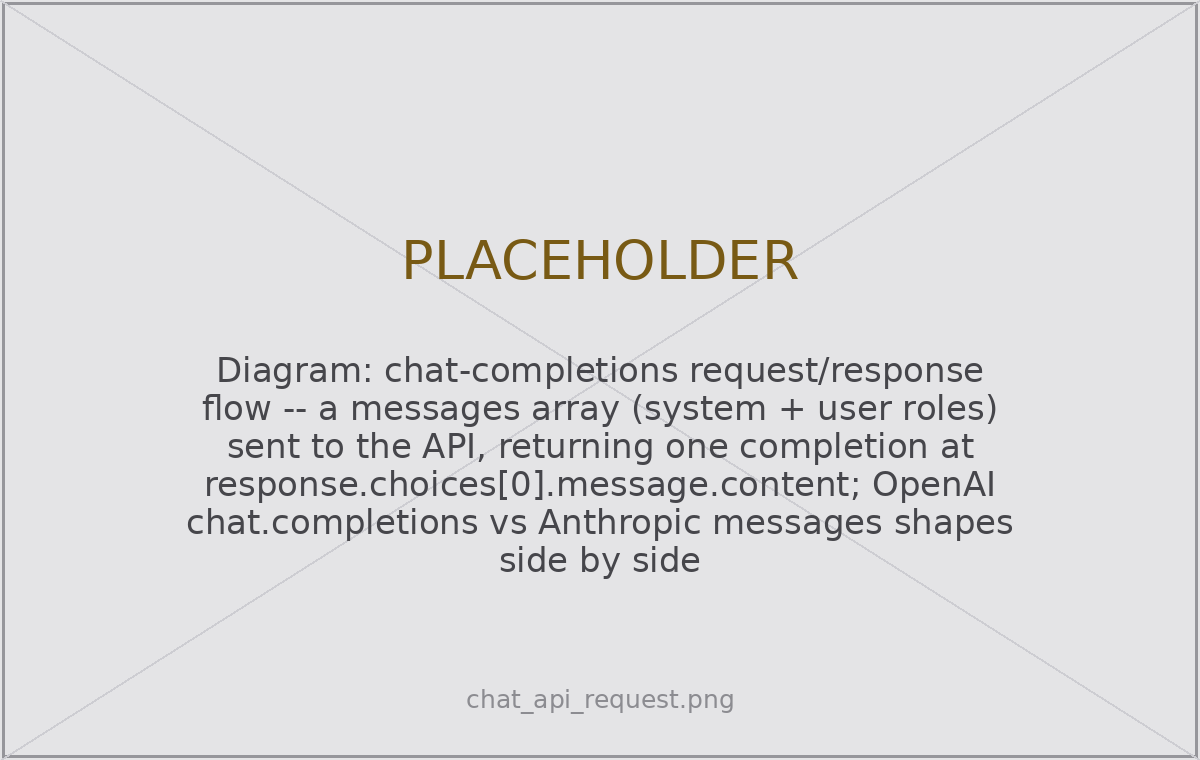
\includegraphics[width=\textwidth]{img/chat_api_request.png}\\
            {\scriptsize Messages in, one completion out.}
        \end{column}
    \end{columns}
    \bottomcite{Textbook Ch.~13, ``The OpenAI API'' \& ``The Anthropic API.''}
\end{frame}

\begin{frame}{From free text to structured data}
    For research you rarely want prose --- you want \textbf{fields you can put in a DataFrame}. Two techniques get you there:
    \begin{columns}[T]
        \begin{column}{0.5\textwidth}
            \begin{block}{Few-shot prompting}
                \footnotesize Show the model examples of the input$\rightarrow$output format you want, then ask it to continue the pattern:
                \begin{quote}\scriptsize
                    \texttt{Summary:} ``\dots teacher salaries.''\\
                    \texttt{Category:} education\\[0.3em]
                    \texttt{Summary:} ``\{new bill\}''\\
                    \texttt{Category:} \_\_\_
                \end{quote}
                Set \texttt{temperature=0} to make classification as repeatable as possible.
            \end{block}
        \end{column}
        \begin{column}{0.5\textwidth}
            \begin{block}{Let the API enforce the schema}
                \footnotesize \textbf{Structured Outputs} accept a JSON Schema and \textit{guarantee} the response conforms --- no more brittle parsing. Lighter-weight JSON mode guarantees valid JSON without a fixed schema; Anthropic gets there via \textbf{tool use}.
            \end{block}
            \vspace{0.3em}
            {\footnotesize Beyond extraction, \textbf{embeddings} turn text into vectors so you can measure \textit{semantic} similarity --- more on Wednesday.}
        \end{column}
    \end{columns}
    \bottomcite{Textbook Ch.~13, ``Structured Output and Few-Shot Prompting'' \& ``Structured Outputs.''}
\end{frame}

\begin{frame}{The catch: non-determinism, cost \& reproducibility}
    \begin{columns}[T]
        \begin{column}{0.56\textwidth}
            When you parse HTML, the same input always gives the same output. LLMs \textbf{break that guarantee}:
            \begin{itemize}\small
                \item Even at \texttt{temperature=0}, outputs vary slightly (floating-point non-determinism)
                \item Model \textbf{weights change} behind a fixed name over time
                \item Retired models make exact replication \textbf{impossible}
            \end{itemize}

            \vspace{0.5em}

            Send the same prompt to two models and they mostly agree --- but \textbf{disagree at the boundaries} (is an EV-incentive bill \texttt{environment} or \texttt{transportation}?). That is genuine ambiguity, not a bug.

            \vspace{0.4em}

            \textbf{Treat the model as a measurement instrument} --- and calibrate it against human judgment.
        \end{column}
        \begin{column}{0.4\textwidth}
            \centering
            
\includegraphics[width=\textwidth]{img/model_comparison.png}\\
            {\scriptsize Two models, one prompt --- agreement is a finding, not a given.}
        \end{column}
    \end{columns}
    \bottomcite{Textbook Ch.~13, ``Reproducibility and Documentation'' \& ``Comparing Model Outputs.'' Connects to the book's AI-disclosure appendix.}
\end{frame}

% =========================================================================
\section{Wednesday · Notebook Lab}
% =========================================================================

\begin{frame}[fragile]{Setup \& your first call}
    Store the key in the environment (never in code), then make one request:
\begin{lstlisting}
import os
from openai import OpenAI

# The key lives in an environment variable -- never in the source
client = OpenAI(api_key=os.environ.get("OPENAI_API_KEY"))

response = client.chat.completions.create(
    model="gpt-4o-mini",
    messages=[
        {"role": "system", "content": "You are a helpful assistant."},
        {"role": "user",   "content": "What is web scraping in one sentence?"},
    ],
)
answer = response.choices[0].message.content   # the model's reply text
\end{lstlisting}
    \bottomcite{Textbook Ch.~13, ``Basic Chat Completion.'' Key storage: \textit{Missing Manual} Ch.~29.}
\end{frame}

\begin{frame}[fragile]{Few-shot classification, one bill at a time}
    Wrap the call in a function; keep the \texttt{sleep} in the \textit{caller}:
\begin{lstlisting}
def classify_bill(summary, client):
    response = client.chat.completions.create(
        model="gpt-4o-mini",
        messages=[
            {"role": "system", "content":
                "Classify this bill into ONE category: education, healthcare, "
                "environment, taxation, criminal_justice, ... or other. "
                "Respond with only the category label."},
            {"role": "user", "content": summary},
        ],
        temperature=0,        # reduce randomness for classification
    )
    return response.choices[0].message.content.strip().lower()
\end{lstlisting}
\begin{lstlisting}
for bill in bills:                       # each bill is a dict with a "summary"
    bill["category"] = classify_bill(bill["summary"], client)
    time.sleep(1)                        # rate-limit between API calls
\end{lstlisting}
    \bottomcite{Textbook Ch.~13, ``Applied Example: Legislative Bill Analysis,'' Step 1.}
\end{frame}

\begin{frame}[fragile]{Get JSON out --- and stop it from breaking}
    The defensive fallback treats bad JSON as a fact of life:
\begin{lstlisting}
# Fallback: ask for JSON, then parse defensively
try:
    extracted = json.loads(response.choices[0].message.content)
except json.JSONDecodeError:
    print("Model did not return valid JSON")   # log it and move on
\end{lstlisting}
    Better --- hand the API a schema and it \textbf{guarantees} the shape:
\begin{lstlisting}
response = client.chat.completions.create(
    model="gpt-4o-mini",
    messages=[{"role": "user", "content": bills[0]["summary"]}],
    response_format={"type": "json_schema", "json_schema": bill_schema},
    temperature=0,
)
result = json.loads(response.choices[0].message.content)  # always parses
\end{lstlisting}
    Anthropic reaches the same guarantee through \textbf{tool use}. Keep the \texttt{try/except} for models that offer no guarantee.
    \bottomcite{Textbook Ch.~13, Step 2 \& ``Structured Outputs: Letting the API Enforce the Format.''}
\end{frame}

\begin{frame}[fragile]{Embeddings: meaning as vectors}
    \begin{columns}[T]
        \begin{column}{0.58\textwidth}
\begin{lstlisting}
def get_embeddings(texts, client,
                   model="text-embedding-3-small"):
    vecs = []
    for text in texts:
        r = client.embeddings.create(
            input=text, model=model)
        vecs.append(r.data[0].embedding)
        time.sleep(0.5)            # rate limit
    return np.array(vecs)

emb = get_embeddings(summaries, client)
# 1.0 == same meaning, 0.0 == unrelated
sim = 1 - cosine(emb[i], emb[j])
\end{lstlisting}
        \end{column}
        \begin{column}{0.4\textwidth}
            \centering
            
\includegraphics[width=\textwidth]{img/embeddings_heatmap.png}\\
            {\scriptsize Bills about ``school funding'' and ``educational resources'' score high despite no shared keywords.}
        \end{column}
    \end{columns}
    \bottomcite{Textbook Ch.~13, ``Text Embeddings'' \& Step 3. Internals: \textit{Missing Manual} Ch.~36.}
\end{frame}

\begin{frame}[fragile]{Two providers, one prompt}
    Send the \textit{identical} classification prompt to Claude and compare:
\begin{lstlisting}
from anthropic import Anthropic
client_a = Anthropic(api_key=os.environ.get("ANTHROPIC_API_KEY"))

# Anthropic: `system` is its own argument; text is response.content[0].text
resp = client_a.messages.create(
    model="claude-sonnet-4-20250514",
    max_tokens=50,
    system=system_prompt,
    messages=[{"role": "user", "content": bill_text}],
)
anthropic_label = resp.content[0].text.strip()

print(openai_label, anthropic_label, openai_label == anthropic_label)
\end{lstlisting}
    Agreement on 85\% of cases is common; the 15\% of disagreements are exactly where you need a human-labeled sample to calibrate.
    \bottomcite{Textbook Ch.~13, ``The Anthropic API'' \& ``Comparing Model Outputs.''}
\end{frame}

\begin{frame}[fragile]{Mind the cost, pin the version}
    \begin{columns}[T]
        \begin{column}{0.56\textwidth}
\begin{lstlisting}
# Estimate BEFORE a big batch.
# gpt-4o-mini ~ $0.15 in / $0.60 out per 1M tok
n_bills = 500
in_tokens  = n_bills * 200   # summary ~200 tok
out_tokens = n_bills * 5     # label   ~5 tok
cost = (in_tokens*0.15 + out_tokens*0.60) / 1e6
print(f"Estimated cost: ${cost:.4f}")
\end{lstlisting}
            {\footnotesize For research, pin the \textbf{dated} model (\texttt{gpt-4o-mini-2024-07-18}) and log every call --- model, full prompt, params, timestamp --- to a JSONL audit trail.}
        \end{column}
        \begin{column}{0.4\textwidth}
            \centering
            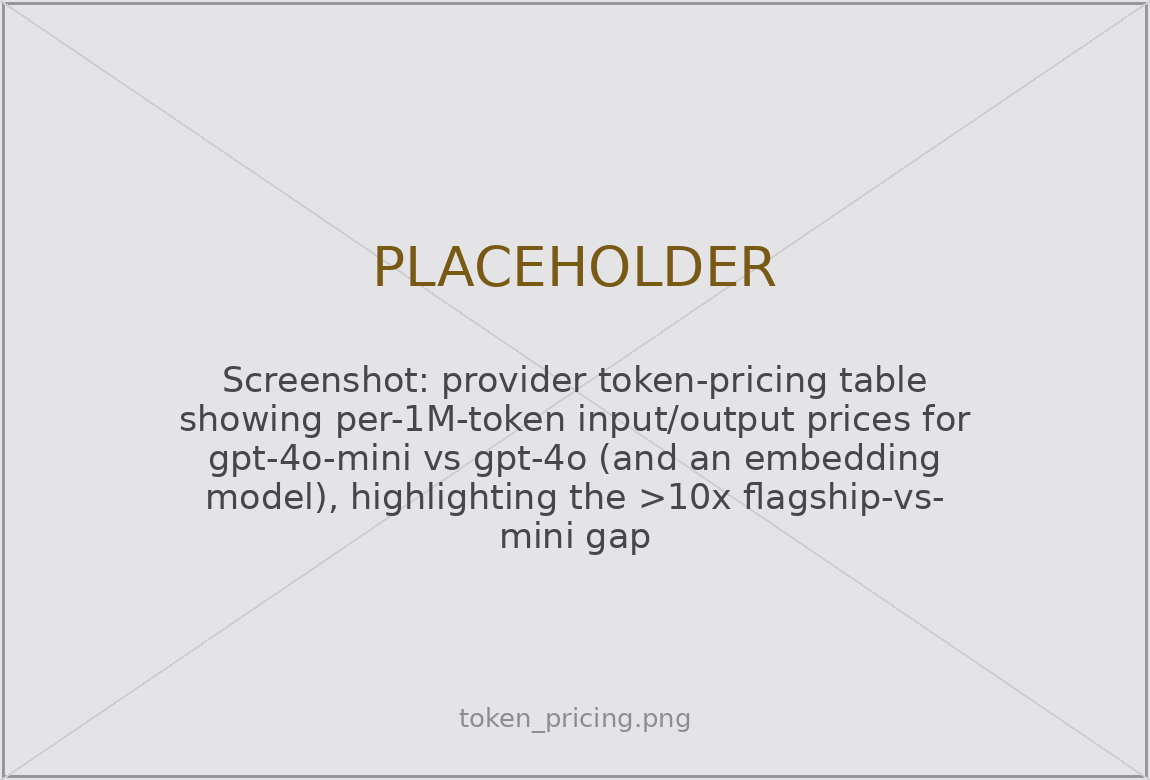
\includegraphics[width=\textwidth]{img/token_pricing.png}\\
            {\scriptsize Flagship models cost $>$10$\times$ their mini siblings. Develop on mini; promote to the big model only after validating prompts.}
        \end{column}
    \end{columns}
    \bottomcite{Textbook Ch.~13, ``Cost Management'' \& ``Reproducibility and Documentation.''}
\end{frame}

\begin{frame}{Lab: work these, then show-and-tell}
    \begin{columns}[T]
        \begin{column}{0.62\textwidth}
            Work through the notebook exercises in pairs:
            \begin{enumerate}\small
                \item Structured extraction from 10+ scraped documents --- design, test, assess quality
                \item Embedding analysis: cluster 20+ documents by cosine similarity; do clusters match intuition?
                \item Human--AI agreement: hand-code 20, then have an LLM classify; where does it disagree?
                \item Cross-model comparison: GPT-4o-mini \textit{vs.}\ Claude on 20 hand-coded samples
                \item Hierarchical clustering: dendrogram of 30 Wikipedia titles across three topics
                \item[6.] \textcolor{tab-purple}{\textbf{5617}}: a validation study \textit{vs.}\ \textcite{ziems2024can} --- 50 items, 25 hand-coded, report Cohen's $\kappa$
            \end{enumerate}
        \end{column}
        \begin{column}{0.34\textwidth}
            \begin{block}{Show-and-Tell}
                \footnotesize Come ready to share:
                \begin{itemize}\footnotesize
                    \item a prompt that surprised you (good or bad)
                    \item interesting extracted data
                    \item a research provocation about LLMs as instruments
                \end{itemize}
            \end{block}
        \end{column}
    \end{columns}
\end{frame}

\begin{frame}[standout]
    An LLM is a measurement instrument, not an oracle.\\
    Same prompt, different model --- different answer.\\[1em]
    Pin the version, log the call, validate against a human.\\[1em]
    {\large Report \textit{what you ran}, not just what you found.}
\end{frame}

% =========================================================================
\section{Friday · Textbook Revisions}
% =========================================================================

\begin{frame}{Improving Chapter 13 together}
    \begin{columns}[T]
        \begin{column}{0.6\textwidth}
            Today we make the book better. Each of you opens a \textbf{pull request} against \texttt{ch-13-ai-apis.qmd} and reviews a classmate's.

            \vspace{1em}

            The workflow (from Week 1):
            \begin{enumerate}\small
                \item Branch / fork the book repo
                \item Edit the chapter; commit with a clear message
                \item Open a PR describing \textit{what} and \textit{why}
                \item Review two peers' PRs: kind, specific, actionable
            \end{enumerate}

            \vspace{0.6em}

            This chapter is \textit{about} AI --- so if an LLM helped you revise it, that is exactly the kind of use the book asks you to \textbf{disclose}.
        \end{column}
        \begin{column}{0.36\textwidth}
            \centering
            
\includegraphics[width=\textwidth]{img/pr_review.png}
        \end{column}
    \end{columns}
    \bottomcite{Contributions \& reviews count toward the Textbook Revisions grade (30\%).}
\end{frame}

\begin{frame}{A revision menu for Chapter 13}
    High-value targets --- pick one and scope it to a single PR:
    \begin{itemize}
        \item \textbf{Re-verify the model names.} The chapter's own ``Model Names Rotate'' callout warns these go stale. Check the providers' current lineups; update names or add a dated note.
        \item \textbf{Deepen ``Common Issues to Debug.''} Add a worked API-key-in-git-history recovery, or a real JSON-parse failure and its \texttt{try/except} fix.
        \item \textbf{Add a figure the prose implies.} A request/response diagram, the token-pricing comparison, or the embedding-similarity heatmap would all help.
        \item \textbf{Contribute a reproducibility helper.} The chapter recommends logging each call to JSONL --- ship a small reusable \texttt{log\_call()} function.
        \item \textbf{Strengthen a thin exercise.} Add expected output, a rubric, or a starter cell so an exercise is self-checking.
        \item \textbf{Extend ``Further Reading.''} An open-weight-models entry (LLaMA, Mistral, Qwen) tied to the access-inequality callout.
    \end{itemize}
    \bottomcite{Targets drawn from the chapter's callouts, ``Common Issues to Debug,'' and ``Further Reading.''}
\end{frame}

\begin{frame}{A good revision, a good review --- and honest disclosure}
    \begin{columns}[T]
        \begin{column}{0.36\textwidth}
            \begin{block}{A strong PR}
                \begin{itemize}\footnotesize
                    \item One focused change, clearly titled
                    \item Explains the problem it fixes
                    \item Renders (\texttt{quarto render}) cleanly
                    \item Matches the book's voice
                \end{itemize}
            \end{block}
            \begin{block}{A strong review}
                \begin{itemize}\footnotesize
                    \item Runs the code, not just skims
                    \item Names specifics; splits must-fix from nice-to-have
                    \item Ends with a clear verdict
                \end{itemize}
            \end{block}
        \end{column}
        \begin{column}{0.6\textwidth}
            \begin{alertblock}{Disclose your AI use}
                \footnotesize The book's \textbf{AI Coauthorship \& Responsible Disclosure} appendix asks four questions --- answer them in your PR when AI helped:
                \begin{enumerate}\footnotesize
                    \item \textbf{What tool?} model \& version (e.g.\ GPT-4o, March 2026)
                    \item \textbf{What task?} drafting prose, generating a code cell, classifying text\dots
                    \item \textbf{What oversight?} how you tested \& verified the output
                    \item \textbf{What limitations?} where you are unsure
                \end{enumerate}
                \vspace{0.2em}
                {\scriptsize Disclosure is about \textit{transparency, not permission} --- and you remain fully accountable for what you submit.}
            \end{alertblock}
        \end{column}
    \end{columns}
    \vspace{0.3em}
    \centering\small Next week: \textbf{Automating data collection} --- schedulers, pipelines, and keeping a scraper alive.
\end{frame}

% =========================================================================
\begin{frame}{Key takeaways}
    \begin{enumerate}
        \item An LLM is \textbf{another API}: authenticate, construct a request, parse the response --- read the docs and manage your keys.
        \item Prompt for \textbf{structure}: few-shot examples, \texttt{temperature=0}, and schema-enforced outputs beat parsing free text.
        \item \textbf{Embeddings} measure semantic similarity where keywords fail --- classify, cluster, and compare at scale.
        \item Non-determinism, cost, and reproducibility are \textbf{real}: estimate spend, pin dated model versions, and log every call.
        \item Treat the model as a \textbf{measurement instrument} --- validate against human judgment and \textbf{disclose} how AI was used.
    \end{enumerate}
    \vspace{1em}
    \bottomcite{Reading: Textbook Ch.~13. Related: \textcite{ziems2024can}; OpenAI \& Anthropic API docs. Disclosure: the AI Coauthorship appendix.}
\end{frame}

\end{document}
